% Created 2013-06-13 Thu 14:35
\documentclass[presentation]{beamer}
\usepackage[utf8]{inputenc}
\usepackage[T1]{fontenc}
\usepackage{fixltx2e}
\usepackage{graphicx}
\usepackage{longtable}
\usepackage{float}
\usepackage{wrapfig}
\usepackage{soul}
\usepackage{textcomp}
\usepackage{marvosym}
\usepackage{wasysym}
\usepackage{latexsym}
\usepackage{amssymb}
\usepackage{amstext}
\usepackage{hyperref}
\tolerance=1000
          \usepackage{listings}\usepackage{fontspec}\usepackage{xunicode}\usepackage{xltxtra}\usepackage{xeCJK}
\setmainfont{Times New Roman}\setmonofont{Courier New}\setCJKmainfont[BoldFont=YouYuan]{SimSun}\setCJKfamilyfont{song}{SimSun}\setCJKfamilyfont{msyh}{微软雅黑}\setCJKfamilyfont{fs}{FangSong}
\usepackage{algorithm}\usepackage{algorithmicx}\usepackage{algpseudocode}\floatname{algorithm}{算法}\renewcommand{\algorithmicrequire}{\textbf{输入:}}\renewcommand{\algorithmicensure}{\textbf{输出:}}
\usepackage{booktabs}\usepackage{pbox}
\AtBeginSection[]{\begin{frame}<beamer>\frametitle{提纲}\tableofcontents[currentsection]\end{frame}}
\usetheme{default}
\author{计92 丘骏鹏 2009011282}
\date{指导老师:朱小燕~ 郝宇}
\title{大数据环境下信息抽取模板自动聚类与发现}
\hypersetup{
  pdfkeywords={},
  pdfsubject={},
  pdfcreator={Emacs 24.2.1 (Org mode 8.0.3)}}
\begin{document}

\maketitle
\begin{frame}<beamer>\frametitle{提纲}\tableofcontents\end{frame}
\section{研究内容介绍}
\label{sec-1}
\begin{frame}[label=sec-1-1]{背景}
\begin{itemize}
\item “大数据”时代来临,我们获得的数据越来越多,研究工作也受到了新的挑战
\item 为了便于计算机处理这些数据,需要从非结构化和半结构化数据中提取出我们关心的内容,
存储成结构化的数据
\item 大部分网页是通过查询后台数据库,然后选择合适模板进行渲染方式生成的,因此可以通
过模板来进行内容的提取。
\begin{figure}[htb]
\centering
\includegraphics[width=0.5\textwidth]{./django.png}
\caption{\label{fig:django}Django中的模板}
\end{figure}
\end{itemize}
\end{frame}

\begin{frame}[label=sec-1-2]{工作内容和特点}
\begin{block}{工作内容}
\begin{itemize}
\item 已经获得大量新闻、博客等网页数据,这些网页可能由不同的模板生成,我们从中提取出
所有可能的模板
\item 根据提取出的模板,抽取新的网页中的有用的信息
\end{itemize}
\end{block}

\begin{block}{特点}
\begin{itemize}
\item 由于我们的数据量比较大,因此需要设计一些高效的算法
\item 海量数据提供了较多的冗余性,弥补算法的一些不精确性
\end{itemize}
\end{block}
\end{frame}

\section{系统框架与模块实现}
\label{sec-2}
\begin{frame}[label=sec-2-1]{整体框架}
\begin{figure}[htb]
\centering
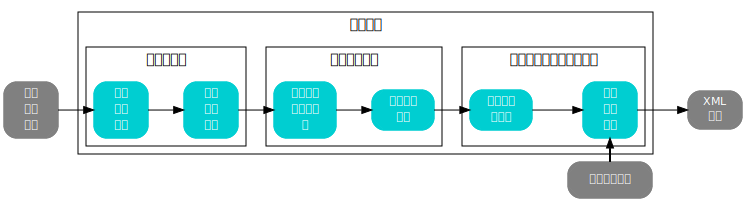
\includegraphics[width=\textwidth]{./framework.pdf}
\caption{\label{fig:framework}整体框架}
\end{figure}
\end{frame}

\begin{frame}[fragile,label=sec-2-2]{预处理模块-过滤无用网页}
 \begin{itemize}
\item 404等错误页大小一般比较小,可以通过设置文件大小阈值过滤
\item 目录页的URL有一定的模式,可以用为每类网页分别建立正则表达式的方法过滤目录页。比
如对于新浪博客来说,详细页的 URL 都以.html 结尾,而目录页则没有。以下两个URL:
\scriptsize
\begin{verbatim}
http://blog.sina.com.cn/u/1439351555
http://blog.sina.com.cn/s/blog_55cac30301016yb1.html
\end{verbatim}
\normalsize
第一个URL对应的是某个博主的文章目录,第二个URL则是该博主的某篇文章。
\end{itemize}
\end{frame}

\begin{frame}[label=sec-2-3]{预处理模块-过滤无用网页}
\begin{itemize}
\item 为了完备性考虑,可能存在某些网站,目录页的 URL 和详细页的 URL 在模式没有太大的区
别,或者人工设置规则的办法太麻烦了
\item 目录页的 HTML 文档的主要部分是由列表环境 <ul> 或 <ol>中的列表项 <li> 及其包含的
超链接标签 <a> 组成。我们提取出网页中的所有<li>标签中的<a>标签,计算这些<a>标签
的文本内容占网页所有文本内容的比重,超过一定的阈值则判定为目录页。
\begin{figure}[htb]
\centering
\includegraphics[width=0.4\textwidth]{./baidunews.png}
\caption{\label{fig:baidunews}百度新闻部分简化的HTML代码}
\end{figure}
\end{itemize}
\end{frame}

\begin{frame}[label=sec-2-4]{预处理模块-简化HTML文档}
\begin{block}{去除无用标签}
\begin{enumerate}
\item 与网页模块无关。去除这些标签时,可以将标签本身及标签的内容一同去
掉。比如 <script>、<link>、<style> 等。
\item 通常是深层次的 HTML 文档的节点,用于控制格式,在模板中意义不大。
去除这些标签时只取出标签本身,保留标签所包含的内容。比如 <br/>、
<p>、<strong>、<em> 等。
\item 我们在实验中不考虑非文本标签,因此将 <img>、<audio> 等直接去除。
\item 最后是去除一些在模板中变化很大的太复杂的标签,典型的是表格相关的
一些标签,包括 <table>、<th>、<tr>、<td> 等。
\end{enumerate}
\end{block}
\end{frame}

\begin{frame}[fragile,label=sec-2-5]{预处理模块-简化HTML文档}
 \begin{block}{对解析好的 DOM Tree 进行简化}
\begin{itemize}
\item 树形结构上做相关的操作较为复杂,我们首先将树形结构转化为更便于处理的序列形式
\item 采用先序遍历的方式,将 DOM Tree 转化成一个标签序列,在遍历的同时在每个节点处
保存了该节点的深度信息
\item 每个标签采用 \texttt{标签名 + 深度} 的表示方法,下图可以表示为:
      \texttt{<html0><body1><div2><a3><p3><div2>}
\includegraphics[width=0.3\textwidth]{./domtree.pdf}
\end{itemize}
\end{block}
\end{frame}

\begin{frame}[label=sec-2-6]{预处理模块-简化HTML文档}
\begin{block}{检测重复记录-后缀树简介}
\begin{itemize}
\item 网页模板中有不定个数的重复模式,通常由模板语言的for语句生成,我们需要将这些记
录合并
\item 后缀树是一种高效的数据结构,可以快速完成重复字串的查找。
\item 后缀树定义:由序列所有的后缀组成的Trie树。后缀树的每一条边都代表着一个序列, 从
根节点到后缀树叶子节点的每条路径都对应着原序列的一个后缀。
\item 后缀树普通的构造算法复杂度很高,系统实现中采用了Ukkonen在1995年提出了一个
  \(O(n)\)时间复杂度的在线构造算法。
\end{itemize}
\end{block}
\end{frame}

\begin{frame}[label=sec-2-7]{后缀树示例}
BANANA对应的的后缀树
\begin{figure}[hb]
\centering
\includegraphics[width=0.5\textwidth]{./suffix-tree-banana.png}
\end{figure}
\end{frame}

\begin{frame}[label=sec-2-8]{后缀树查找重复序列算法}
\begin{block}{原始算法}
\begin{itemize}
\item 任意一条从根节点到内部节点的路径组成的序列都是原序列中重复出现的字串,且重复的次
数是以该内部节点为根的子树的叶子节点个数。
\item 不能处理:不同的重复子串之间可包含或者相交的关系;同一个重复子串在原序列上有交
集
\end{itemize}
\end{block}

\begin{block}{新的算法要求}
\begin{itemize}
\item 重复序列不能横跨两个子树
\item 重复序列必须有公共的父亲
\item 重复序列必须尽可能地长
\end{itemize}
\end{block}
\end{frame}

\begin{frame}[label=sec-2-9]{后缀树查找重复序列算法}
\begin{algorithm}[H]
  \caption{从根节点出发,找出所有的重复子序列\label{suffixtree:algo:fromroot}}
  \begin{algorithmic}[1]
    \Require 已经构建好的后缀树,根为$root$
    \Ensure 该后缀树中所有的重复子序列
    \State $//$从根节点出发,寻找所有的重复子序列
    \For{$edge \gets root.edges~\mathbf{if}~edge.endNode.isNotLeaf$}
    \State $//$取后缀树根节点的每条边的第一个元素作为每个子树的根节点
    \State $subTreeRoot := edge.firstElement$
    \State $//$查找以该节点为根的所有重复子序列
    \State findAllRepetitions$(root, \mathbf{nil}, subTreeRoot)$
    \EndFor
  \end{algorithmic}
\end{algorithm}
\end{frame}

\begin{frame}[label=sec-2-10]{后缀树查找重复序列算法}
\floatname{algorithm}{\tiny 算法}
  \begin{algorithm}[H]
  \caption{\tiny 简化的findAllRepetitions实现}
  \label{suffixtree:algo:findrep}
  \begin{algorithmic}
    \tiny
    \Require 一个内部节点$node$,当前已经找到的重复序列$prefix$,要找的
    子树的根节点$subTreeRoot$
    \Ensure 所有经过该内部节点的符合要求的重复序列
    \Function {findAllRepetitions}{$node, prefix, subTreeRoot$}
    \State $//$定义一个空集合
    \State $results := Collection.empty$
    \State $//$对于该内部节点的每一条不连接叶子节点的边
    \For{$edge \gets node.edges~\mathbf{if}~edge.endNode.isNotLeaf$}
    \State $//$依次取出该条边上属于该根节点子树上的点
    \State $seq := edge.takeWhile(element$ inSubTreeOf $subTreeRoot)$\label{suffixtree:code:equals}
    \If {$seq.length == edge.length$}
    \State $//$遍历完了该条边上所有元素,
    \State $//$则取该条边连接的下一个内部节点进行递归查找
    \State findAllRepetitions($edge.endNode, prefix + seq, subTreeRoot$)
    \Else
    \State $//$否则,将当前得到的序列加入到结果集合中
    \State addToResults$(prefix + seq, results)$\label{suffixtree:code:add}
    \EndIf
    \EndFor
    \State \Return{$results$}
    \EndFunction
    \State
  \end{algorithmic}
\end{algorithm}
\end{frame}

\begin{frame}[fragile,label=sec-2-11]{合并重复记录}
 \begin{itemize}
\item 所有序列按实际的父节点分组,然后对每个分组进行合并,保证重复串有公共的父亲。
\item 但是仍然存在序列相交的情况,如
\scriptsize
\texttt{<div3><div4><div3><div4><a5><img5><div4><a5><img5>}
\normalsize
\texttt{<div3><div4>} 和 \texttt{<div4><a5><img5>} 都是符合算法要求的重复串,但互相之间有
交集 \texttt{<div4>} 。我们采取的策略是只取更深的重复序列。这里只取 \texttt{<div4><a5><img5>}
\end{itemize}
\end{frame}

\begin{frame}[label=sec-2-12]{网页聚类模块-计算结构相似度}
\begin{itemize}
\item 序列 $S_1,S_2$ ,$x_i$ 和 $y_j$ 分别表示 $S_1$ 的第 $i$ 个元素和 $S_2$ 的第
$j$ 个元素, $f(depth)$ 是根据深度加权的函数,我们认为深度越深的节点,成为模板
的概率就越小。
\begin{eqnarray}
t(i)(j) =
\begin{cases}
0 & i = 0,\: j = 0\\
t(i-1)(j-1) + f(x_i.depth) & i,\: j > 0, x_i=y_j\\
\max(t(i)(j-1), t(i-1)(j)) & i, j > 0,\: x_i \ne y_j
\end{cases}
\end{eqnarray}
\item 结构相似度计算公式
  \[
  Sim(D_1,D_2)=\frac{|elcs(S_1,S_2)|}{\max(\sum\limits_{n\in
  S_1}{f(n.depth)},\sum\limits_{n\in S_2}{f(n.depth)})}
  \]
\end{itemize}
\end{frame}

\begin{frame}[label=sec-2-13]{计算时间优化}
\begin{itemize}
\item 文档数量多,计算量很大,需要一定的优化。
\item 采用Actor库实现多线程计算,加快计算速度。将任务分割后交给每个Actor进行计算,
Actor的调度的算法采用RoundRobin。
\item 任务分割示意图
\begin{figure}[hb]
  \centering
  \includegraphics[width=0.35\textwidth]{triangle.jpg}
\end{figure}
\end{itemize}
\end{frame}
\begin{frame}[label=sec-2-14]{聚类算法}
\begin{columns}
\begin{column}{0.4\textwidth}
\begin{enumerate}
\item 初始时,让每个文档实例都单独为一类
\item 迭代时,每次选择距离最近的两个类合并
\item 直到任意两个类的距离都大于阈值时程序退出
\item 算法的结束条件由阈值决定,无需实现设定类的个数。
\end{enumerate}

\end{column}

\begin{column}{0.5\textwidth}
\includegraphics[width=\textwidth]{./aggloclustering.png}

\end{column}
\end{columns}
\end{frame}

\begin{frame}[label=sec-2-15]{模板形式化定义}
\begin{block}{基本节点}
\begin{itemize}
\item 两种组成方式 
\begin{enumerate}
\item 单个不重复的HTML标签,即 $<tag>$
\item 由一个或多个HTML标签组成的序列,这些序列可以出现一次或多次,即
         $(\sum_{i=1}^N<tag_i>)+$ ,其中 $N \ge 1$
\end{enumerate}
\item 第二种形式通过合并重复记录得到,对应的模板语言为:
\begin{figure}[hb]
\centering
\includegraphics[width=0.4\textwidth]{django-for}
\end{figure}
\item 还有一种模板生成形式:
\begin{figure}[hb]
\centering
\includegraphics[width=0.35\textwidth]{django-if}
\end{figure}
\end{itemize}
\end{block}
\end{frame}
\begin{frame}[label=sec-2-16]{模板形式化定义}
\begin{block}{必选和可选节点}
\begin{itemize}
\item 必选节点 $EN$ 对应着由基本节点组成的一个序列,若模板节点用 $tn_i$ 表示,则必
选节点可以表示为
\[
      EN=tn_1tn_2...tn_n
      \]
\item 可选节点 $ON$ 同时对应多个序列,每个序列由不同的基本节点组成,同时每个序列
还对应着一个出现概率 $p$ ,即:
\[
      ON=tn_{11}tn_{12}...tn_{1n_1},p_1|tn_{21}tn_{22}...tn_{2n_2},p_2|...|tn_{k1}tn_{k2}...tn_{kn_k},p_k
      \]
\item 定义模板 $Tp$ 必须由这两种节点交替组成:
      \[
      Tp=[ON_0]EN_1ON_1EN_2ON_2......EN_n[ON_n] 
      \]
\end{itemize}
\end{block}
\end{frame}

\begin{frame}[label=sec-2-17]{模板生成算法}
\begin{itemize}
\item 找出所有组成必选节点的基本节点:对于一个聚类的全部序列,从聚类中心点开始,
依次计算一次最长公共子序列,得到 $n$ 个序列的公共子序列 $S_{common}$
\item 每个序列和 $S_{common}$ 对齐,得到一些未对齐的区间,每个未对齐的区间计算一个
可选节点
\item 已对齐的基本节点组成必选节点
\item 必选节点和可选节点交替出现,组成最终的模板
\end{itemize}
\end{frame}

\begin{frame}[label=sec-2-18]{模板生成流程图}
\includegraphics[width=0.7\textwidth]{./subsystem.png}
\end{frame}

\begin{frame}[label=sec-2-19]{简单的例子}
\begin{itemize}
\item 设有3个序列,分别为:
\begin{eqnarray*}
s_1&=&aorzbcdlxe\\
s_2&=&athubeatcdlxe\\
s_3&=&athubeatcdpkue
\end{eqnarray*}
\item 根据最长公共子串算法,得到 $s_{common}$ 为 $abcde$
\item 每个序列同 $s_{common}$ 进行对齐,得到
\begin{matrix}
s_1      &:&\mathbf{a}&orz&\mathbf{b}&   &\mathbf{cd}&lx&\mathbf{e}\\
s_2      &:&\mathbf{a}&thu&\mathbf{b}&eat&\mathbf{cd}&lx&\mathbf{e}\\
s_3      &:&\mathbf{a}&thu&\mathbf{b}&eat&\mathbf{cd}&pku&\mathbf{e}\\
s_{common}&:&\mathbf{a}&   &\mathbf{b}&   &\mathbf{cd}&   &\mathbf{e}
\end{matrix}
\end{itemize}
\end{frame}

\begin{frame}[label=sec-2-20]{简单的例子}
\begin{itemize}
\item 根据上述对齐结果,生成以下可选节点:
\begin{eqnarray*}
ON_{a,b}&=&thu,2/3~|~orz,1/3\\
ON_{b,c}&=&eat,2/3\\
ON_{d,e}&=&lx,2/3~|~pku,1/3
\end{eqnarray*}
\item 对齐的部分则对应生成必选节点,注意将连续的基本节点合并,分别为: $a,b,cd,e$
\end{itemize}
\end{frame}

\begin{frame}[label=sec-2-21]{可选节点生成的实际实现}
\begin{itemize}
\item 实际情况要比上面的例子复杂。区间 $[t1,t2]$ 中未对齐的那些标签子序列,有些可能差
异很大,有些则可能非常相近,但不完全一样。
\item 我们发现,解决构造可选节点的这个子问题和模板提取的问题的流程都可以简单描述为:
\\
\textbf{\scriptsize
存在一个序列集合,元素由几种不同的模式生成,先将这些元素分成几种类别,然后针
对每个类别去提取“模板”}
\item 因此,我们可以使用一个“自相似”的框架解决可选节点生成问题。下面,我们把成为构
造可选节点时需要提取的公共的模式称为“子模板”。
\end{itemize}
\end{frame}

\begin{frame}[label=sec-2-22]{构造可选节点流程}
\includegraphics[width=0.75\textwidth]{./subtemplate.png}
\end{frame}

\begin{frame}[label=sec-2-23]{内容提取模块}
\begin{columns}
\begin{column}{0.55\textwidth}
\begin{enumerate}
\item 针对每个模板做一些简单的人工标注,如新闻网页模板的标题,正文,评论等
\item 判断新输入的网页属于哪个聚类,选择对应的模板
\item 模板与网页的序列对齐,根据标注抽取我们感兴趣的部分
\end{enumerate}

\end{column}

\begin{column}{0.4\textwidth}
\includegraphics[width=\textwidth]{./extractor.png}

\end{column}
\end{columns}
\end{frame}

\begin{frame}[label=sec-2-24]{模板匹配演示系统}
\begin{itemize}
\item 基于Play! Framework(Scala)实现了一个Web Service
\includegraphics[width=0.6\textwidth]{./demo.png}
\end{itemize}
\end{frame}
\section{实验和分析}
\label{sec-3}
\begin{frame}[label=sec-3-1]{实验环境和数据}
\begin{itemize}
\item 机器的配置情况是:16个逻辑核的CPU,24G内存,操作系统为64位的CentOS。
\item 数据统计
\begin{table}[h]
\centering
\begin{tabular}{llll}
\toprule
& blog & news & other \\
\hline
文件个数 & 59998 & 81561 & 183635 \\
总大小 & 5.4G & 7.9G & 18G \\
来源 & blog.sina.com.cn &  news.xxx.com &  \\
\bottomrule
\end{tabular}
\end{table}
\end{itemize}
\end{frame}

\begin{frame}[label=sec-3-2]{预处理模块}
\begin{itemize}
\item 过滤目录页的规则
\end{itemize}
\begin{table}[hb]
  \centering
  \begin{tabular}{lrrr}
    \toprule
    & blog & news & others \\
    \hline
    目录页URL规则 & .*(?<!\textbackslash\textbackslash.html?)\$ & .*(?<!\textbackslash\textbackslash.shtml)\$ &  \\
    错误页最大长度 & 6000 & 6000 &  \\
    文件个数 & 59998 & 81561 & 183635 \\
    过滤后详细页个数 &  &  &  \\
    \bottomrule
  \end{tabular}
\end{table}
\begin{itemize}
\item 训练集和测试集分割
\begin{table}[hb]
  \centering
  \begin{tabular}{llll}
    \toprule
    & 训练集 & 测试集 & 详细页总数 \\
    \hline
    blog &  &  &  \\
    news &  &  &  \\
    others &  &  &  \\
    \bottomrule
  \end{tabular}
\end{table}
\end{itemize}
\end{frame}

\begin{frame}[label=sec-3-3]{预处理模块}
\begin{block}{无用标签去除规则}
\begin{table}[hb]
  \centering
  \begin{tabular}{ll}
    \toprule
    正则表达式模式 & 对应的标签名 \\
    \hline
    (?is)<tag.*?>.*?</tag> & style,script \\
    (?is)<[/]?tag.*?> & link,input,br,img,meta,wbr \\
    (?is)<[/]?tag.*?> & strong,em,font,b,p,table \\
    \bottomrule
  \end{tabular}
\end{table}   
\end{block}

\begin{block}{检测出的重复记录统计}
\begin{figure}[hb]
  \centering
  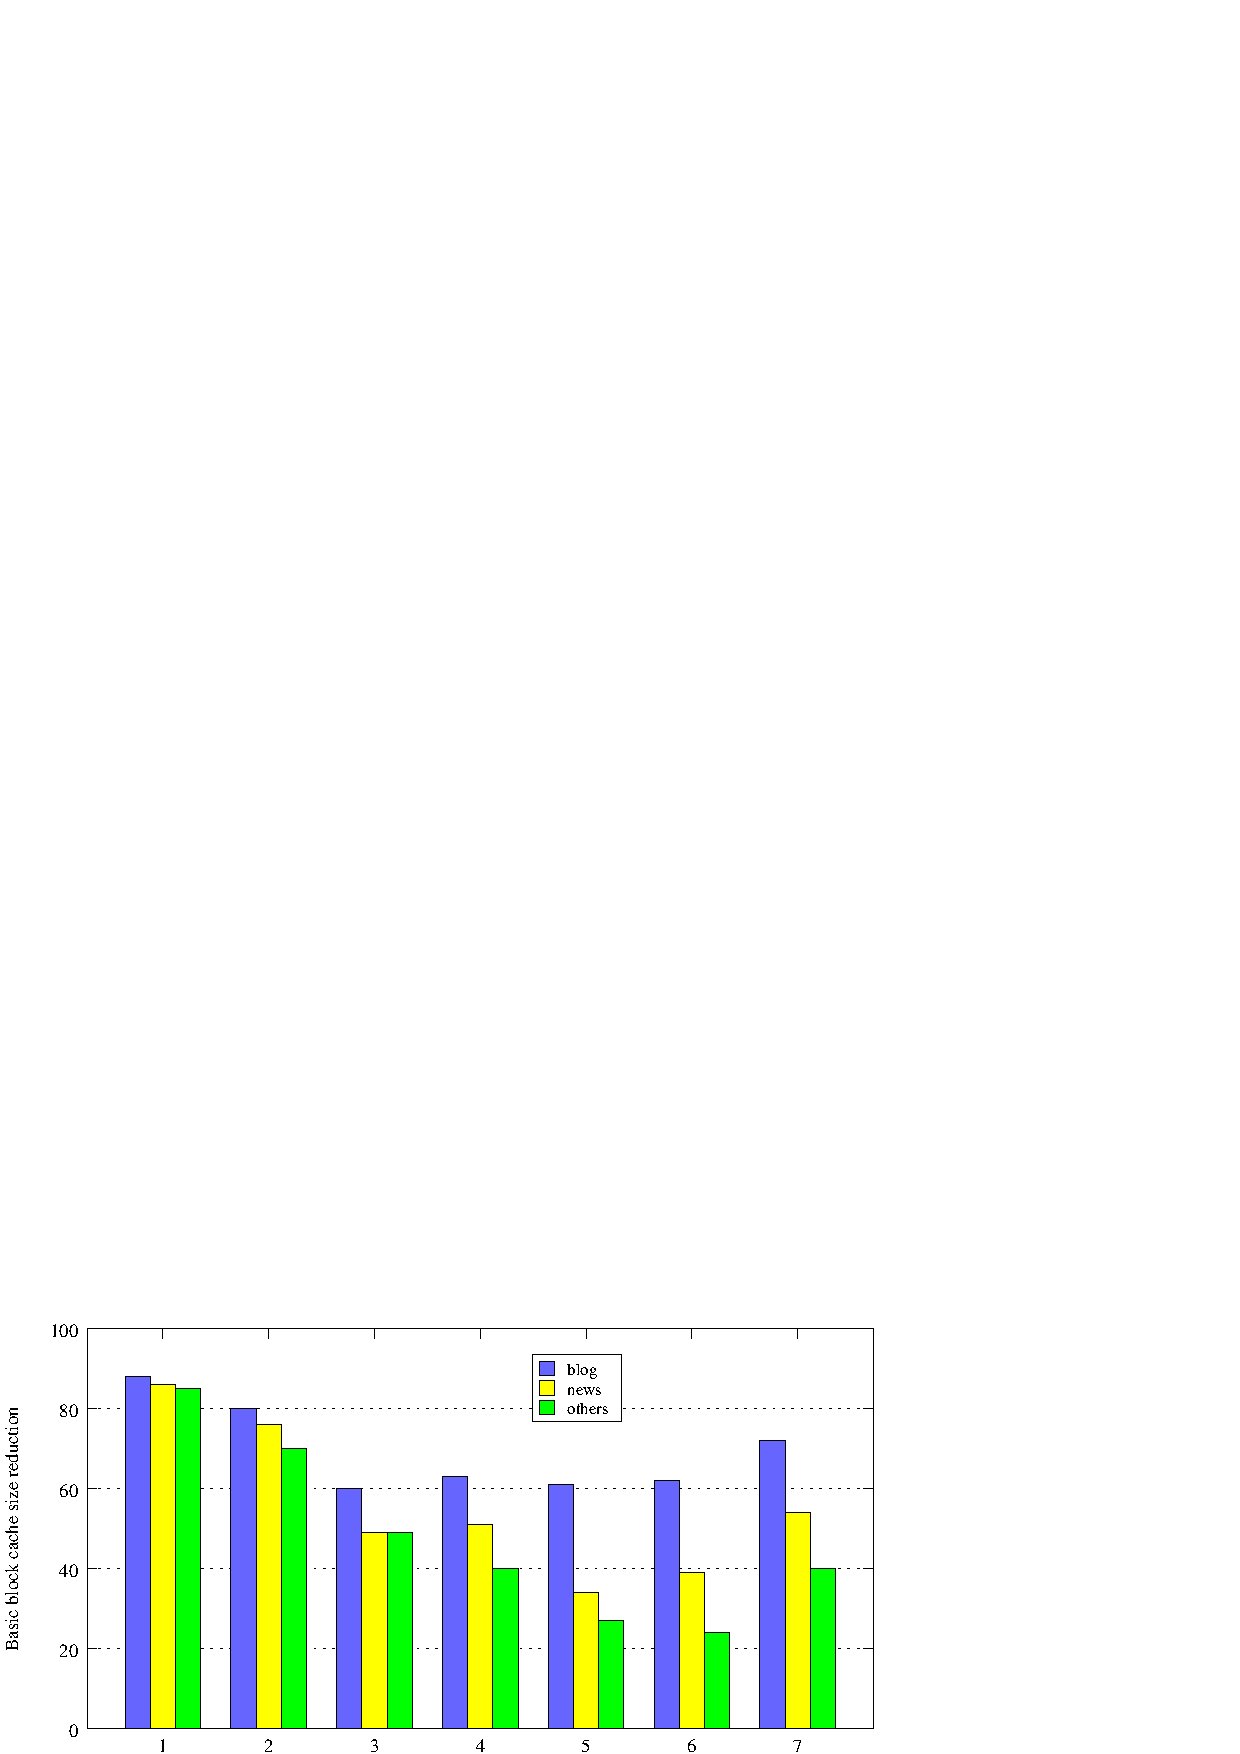
\includegraphics[width=0.6\textwidth]{recordlength.png}
\end{figure}    
\end{block}
\end{frame}

\begin{frame}[label=sec-3-4]{聚类和模板提取}
\begin{itemize}
\item 选择news数据集做实验,调整聚类时的阈值,观察聚类结果
\begin{table}
  \centering
  \begin{tabular}{rllll}
    \toprule
    阈值 & 聚类个数 & 模板长度 & \pbox{2.5in}{必选节点包\\ 含的点数} & \pbox{2.5in}{可选节点\\ 平均长度} \\
    \hline
    0.3 &  &  &  &  \\
    0.4 &  &  &  &  \\
    0.5 &  &  &  &  \\
    0.6 &  &  &  &  
    \bottomrule
  \end{tabular}
\end{table}
\item TODO: 结果分析
\end{itemize}
\end{frame}

\begin{frame}[label=sec-3-5]{提取效果}
\begin{itemize}
\item 我们在测试集上运行我们的程序,抽取出我们需要的信息,并将其保存为XML格式输出。
\begin{figure}[hb]
\centering
\includegraphics[width=0.5\textwidth]{xmloutput}
\end{figure}
\item TODO: 结果统计和分析
\end{itemize}
\end{frame}

\begin{frame}[label=sec-3-6]{演示系统}
\begin{itemize}
\item 模板匹配演示系统的运行效果如下:
\begin{figure}[hb]
  \centering
  \includegraphics[width=0.6\textwidth]{demoresult}
\end{figure}
\end{itemize}
\end{frame}

\section{总结和展望}
\label{sec-4}
\begin{frame}[label=sec-4-1]{总结}
\begin{enumerate}
\item 设计并实现了一个完整的系统,做了很多优化;实现了较高程度的自动化处理,减小人工
参与的工作量。
\item 高效地实现了后缀树这个数据结构,在此基础上设计了一套适用于在树的先序遍历序
列中查找重复子树的算法。
\item 实现并改进了最长公共子序列算法,将其用于计算文档的结构相似度;实现了简单的
凝聚层次聚类算法,并将其用于文档的聚类
\item 实现了一个无监督的模板生成算法,通过人工指定模板中某些部分对应的语义,可以
使用模板提取新的由该模板生成的网页中对应的信息。
\item 实现了一个Web Service,可以直观地看到网页和模板的匹配情况。
\end{enumerate}
\end{frame}
\begin{frame}[label=sec-4-2]{未来的工作}
\begin{enumerate}
\item 预处理模块:改进Ukkonen原有的在线构造算法,在构造树的时候就考虑一些原本的结构
信息。查找重复时利用后缀树中其他的一些信息,比如后缀链。
\item 网页结构相似度计算和网页聚类模块:可以进一步改进计算相似度的算法,加入一些其他
的除了深度之外的更多结构信息;可以考虑使用更复杂但是鲁棒性更好的一些聚类算法。
\item 模板生成和内容提取:对模板生成算法做一些修改,设计一些更高级的机器学习算法。在
内容提取的时候,可以采用树的匹配算法而不是序列的匹配算法。
\end{enumerate}
\end{frame}
% Emacs 24.2.1 (Org mode 8.0.3)
\end{document}